\documentclass[conference]{IEEEtran}
\IEEEoverridecommandlockouts
\usepackage{cite}
\usepackage{amsmath,amssymb,amsfonts}
\usepackage{algorithmic}
\usepackage{graphicx}
\usepackage{textcomp}
\usepackage{xcolor}
\usepackage{booktabs}
\usepackage{hyperref}
\usepackage{tabularx}
\usepackage{multirow}

\def\BibTeX{{\rm B\kern-.05em{\sc i\kern-.025em b}\kern-.08em
    T\kern-.1667em\lower.7ex\hbox{E}\kern-.125emX}}

\begin{document}

\title{Design of a Business Intelligence System Based on a Rule-Based Chatbot with Time Series Forecasting and Natural Language Technology for Business Performance Analysis and Prediction\\
}

\author{\IEEEauthorblockN{Thalita Zahra Sutejo}
\IEEEauthorblockA{\textit{Program Studi Sistem dan Teknologi Informasi} \\
\textit{Sekolah Teknik Elektro dan Informatika, Institut Teknologi Bandung}\\
Bandung, Indonesia \\
18222023@std.stei.itb.ac.id}
}

\maketitle

\begin{abstract}
The exponential growth of data in the telecommunications sector necessitates the development of agile and accessible Business Intelligence (BI) systems. Traditional BI dashboards, while comprehensive, often exhibit steep learning curves and lack seamlessly integrated predictive capabilities. This paper presents "BrightAI," a conversational Business Intelligence framework engineered to integrate a deterministic rule-based chatbot architecture with advanced Time Series Forecasting and Natural Language Generation (NLG). Designed to provide predictive analytics across core domains (sales, revenue, target realization, churn), the system employs a three-tier microservices architecture. The architecture comprises a React-based Frontend Layer, a Node.js Backend Layer implementing a confidence-weighted Natural Language Understanding (NLU) rule engine, and a Python-based FastAPI analytical layer for predictive modeling. The analytical layer evaluates ARIMA, Prophet, LSTM, and GRU models. These models are rigorously validated against strict evaluation protocols utilizing metrics including MAE, RMSE, sMAPE, MASE, and Skill Score. Empirical results demonstrate that the implemented models satisfy predefined Key Performance Indicators (KPIs), achieving an sMAPE of $<30\%$ and a Skill Score of $>0.20$. Furthermore, the algorithmic NLG module accurately translates historical data and forecasted outcomes into coherent executive narratives, thereby significantly optimizing the data-driven decision-making lifecycle.
\end{abstract}

\begin{IEEEkeywords}
Business Intelligence, Chatbot, Time Series Forecasting, Natural Language Generation, Machine Learning
\end{IEEEkeywords}

\section{Introduction}
In contemporary enterprise environments, data constitutes a pivotal asset for strategic operational planning \cite{gul2023from}. Major telecommunications providers oversee vast, complex datasets pertaining to enterprise products, such as High-Speed Internet services. Extracting actionable intelligence from these massive Enterprise Data Warehouses (EDW) traditionally requires intricate Business Intelligence (BI) dashboards or specialized queries, leading to substantial latency.

To maintain a competitive advantage, modern executive operations demand systems that provide not only retrospective data analysis for current data but also proactive predictive forecasting within an intuitive interface. While conventional BI platforms aggregate historical metrics, they frequently lack the conversational interactivity and embedded machine learning necessary for rapid strategic assessments \cite{shah2025hybrid}.

\begin{figure}[htbp]
\centerline{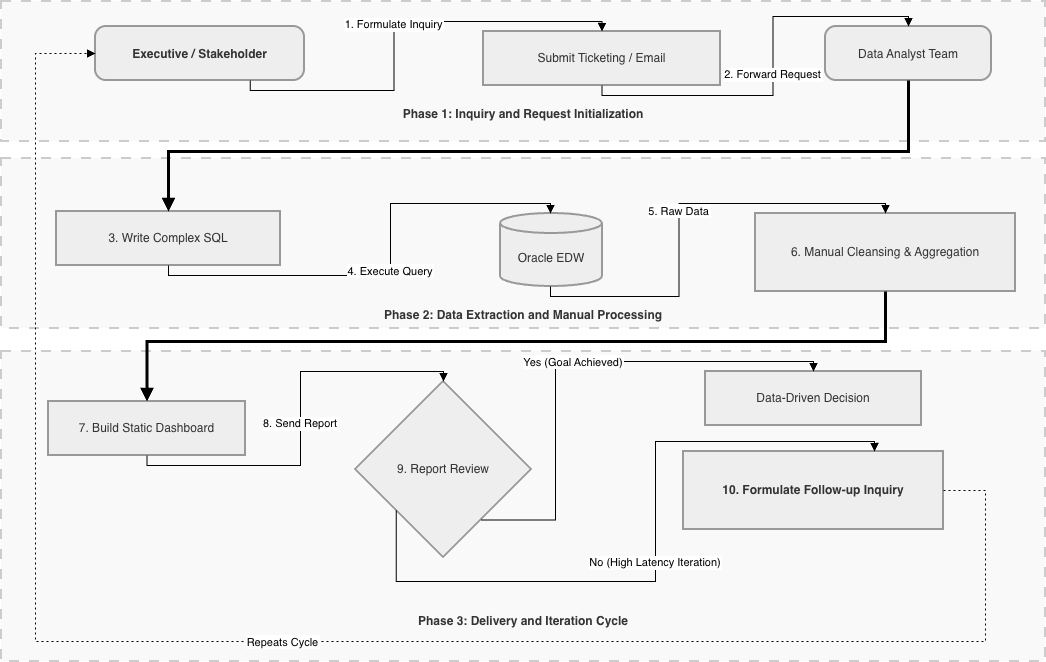
\includegraphics[width=\linewidth,height=4.8cm,keepaspectratio]{asis.png}}
\caption{The As-Is existing business process flow requiring manual BI queries.}
\label{fig:asis}

\end{figure}

As illustrated in Fig.~\ref{fig:asis}, the existing ("As-Is") enterprise business process relies heavily on a fragmented methodology. Decision-makers must manually submit ad-hoc queries to data analysts, who then extract, transform, and process the data. This sequential dependency introduces substantial bottlenecks, hindering the rapid execution of real-time operational strategies.

\begin{figure}[htbp]
\centerline{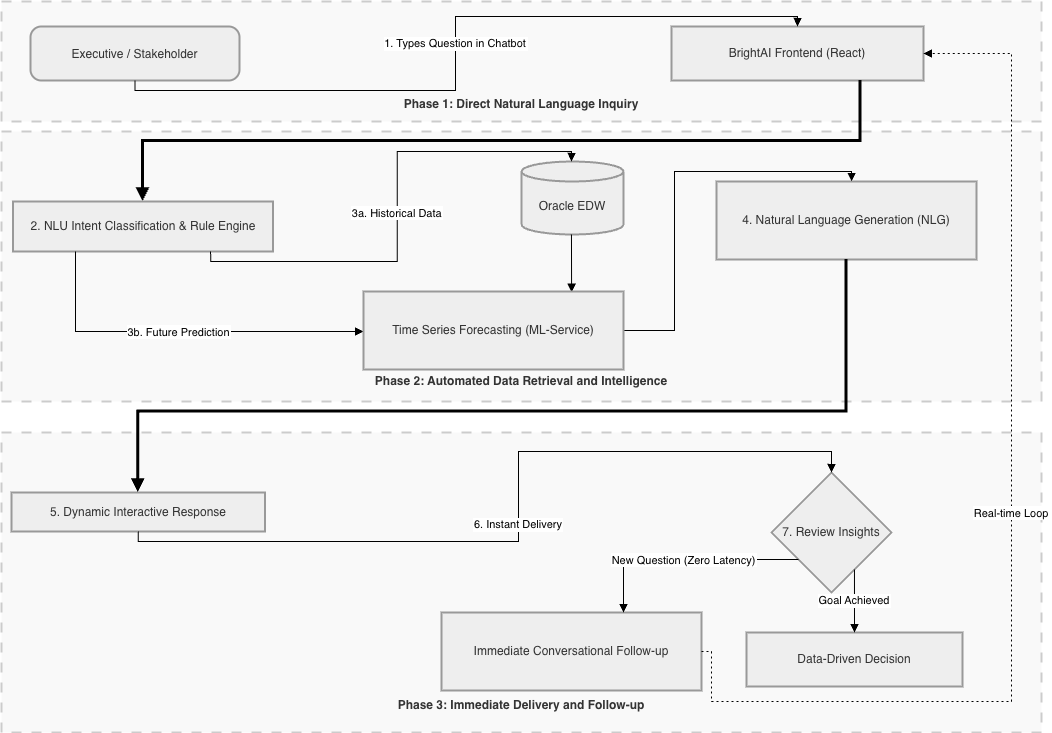
\includegraphics[width=\linewidth,height=4.8cm,keepaspectratio]{tobe.png}}
\caption{The To-Be transformed business process flow via the BrightAI System.}
\label{fig:tobe}
\vspace{-0.3cm}
\end{figure}

Conversely, as illustrated in Fig.~\ref{fig:tobe}, the proposed ("To-Be") BrightAI framework transforms this workflow. By synthesizing a deterministic chatbot interface with Time Series Forecasting and Natural Language Generation (NLG), stakeholders can directly interrogate enterprise databases using natural language. The system dynamically executes complex queries regarding revenue trajectories, sales growth, and customer churn, eliminating the middleman and accelerating data retrieval.

\section{System Architecture}
To guarantee scalability and efficiency, BrightAI implements a modern three-tier microservices framework.

\begin{figure}[htbp]
\centerline{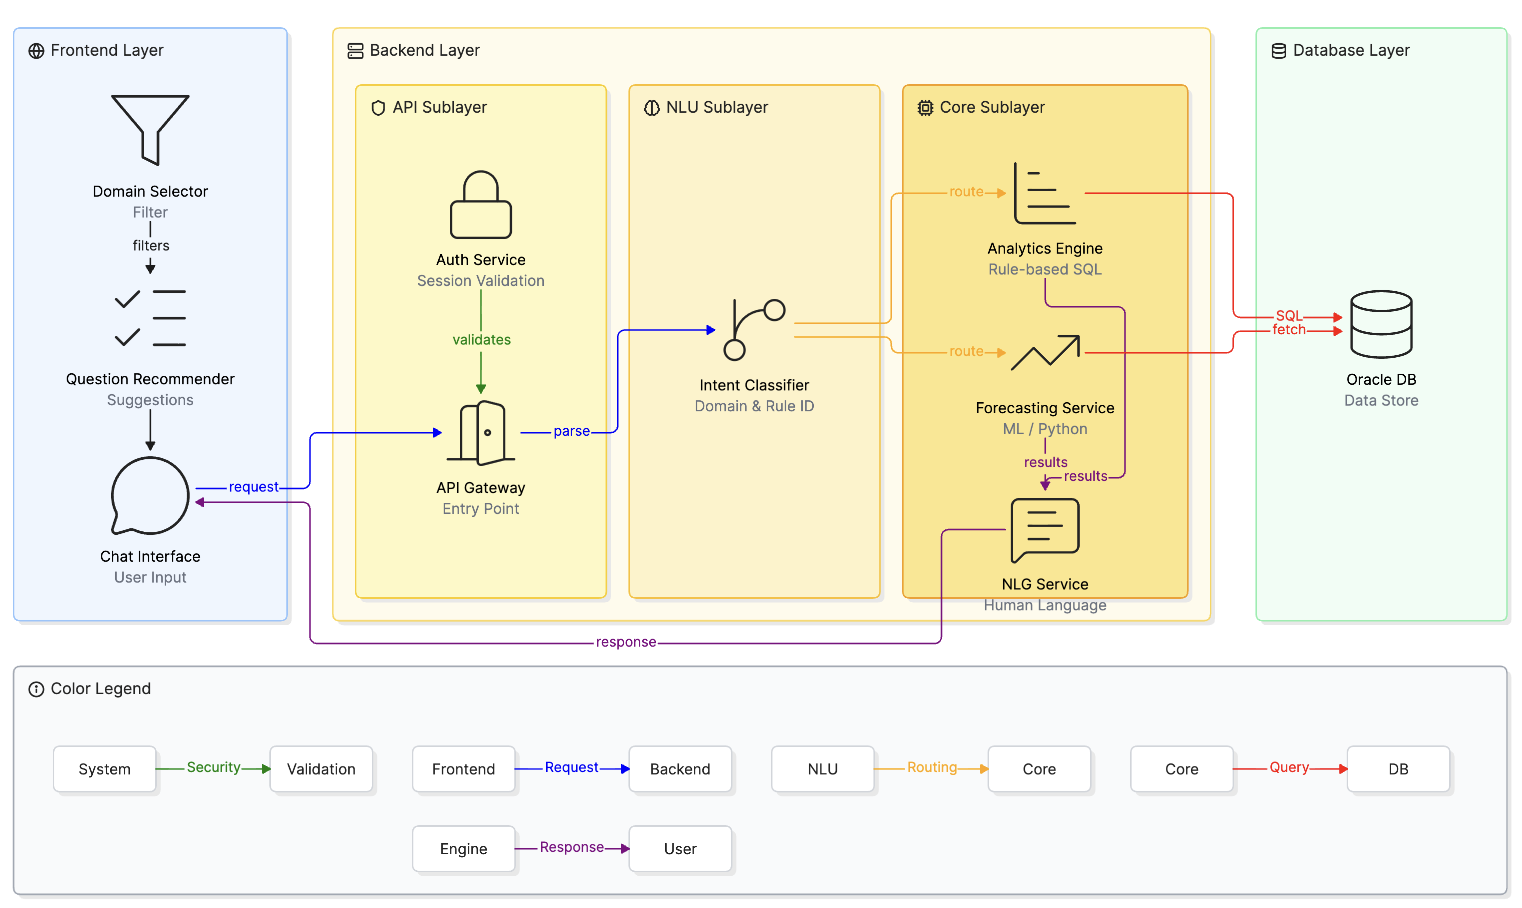
\includegraphics[width=\linewidth,height=4.8cm,keepaspectratio]{ars1.png}}
\caption{The BrightAI overall three-tier microservices architecture integrating React, Node.js, and FastAPI.}
\label{fig:ars1}
\vspace{-0.3cm}
\end{figure}

As illustrated in Fig.~\ref{fig:ars1}, the overall system is structurally divided into three interoperable layers: the Frontend Layer, the Backend Layer, and the Database Layer. This separation ensures intensive predictive processes do not degrade interface responsiveness.

\subsection{Frontend Layer}
Developed utilizing React.js, the frontend serves as the primary user interface. It is architected to simulate a standard messaging application. It parses JSON payloads from the backend to display structured tabular data and textual narratives to the user.

\subsection{Backend Layer}
The backend layer is internally partitioned into three modular sublayers. The API Sublayer, engineered with Node.js and Express, functions as the secure entry point. 

\begin{figure}[htbp]
\centerline{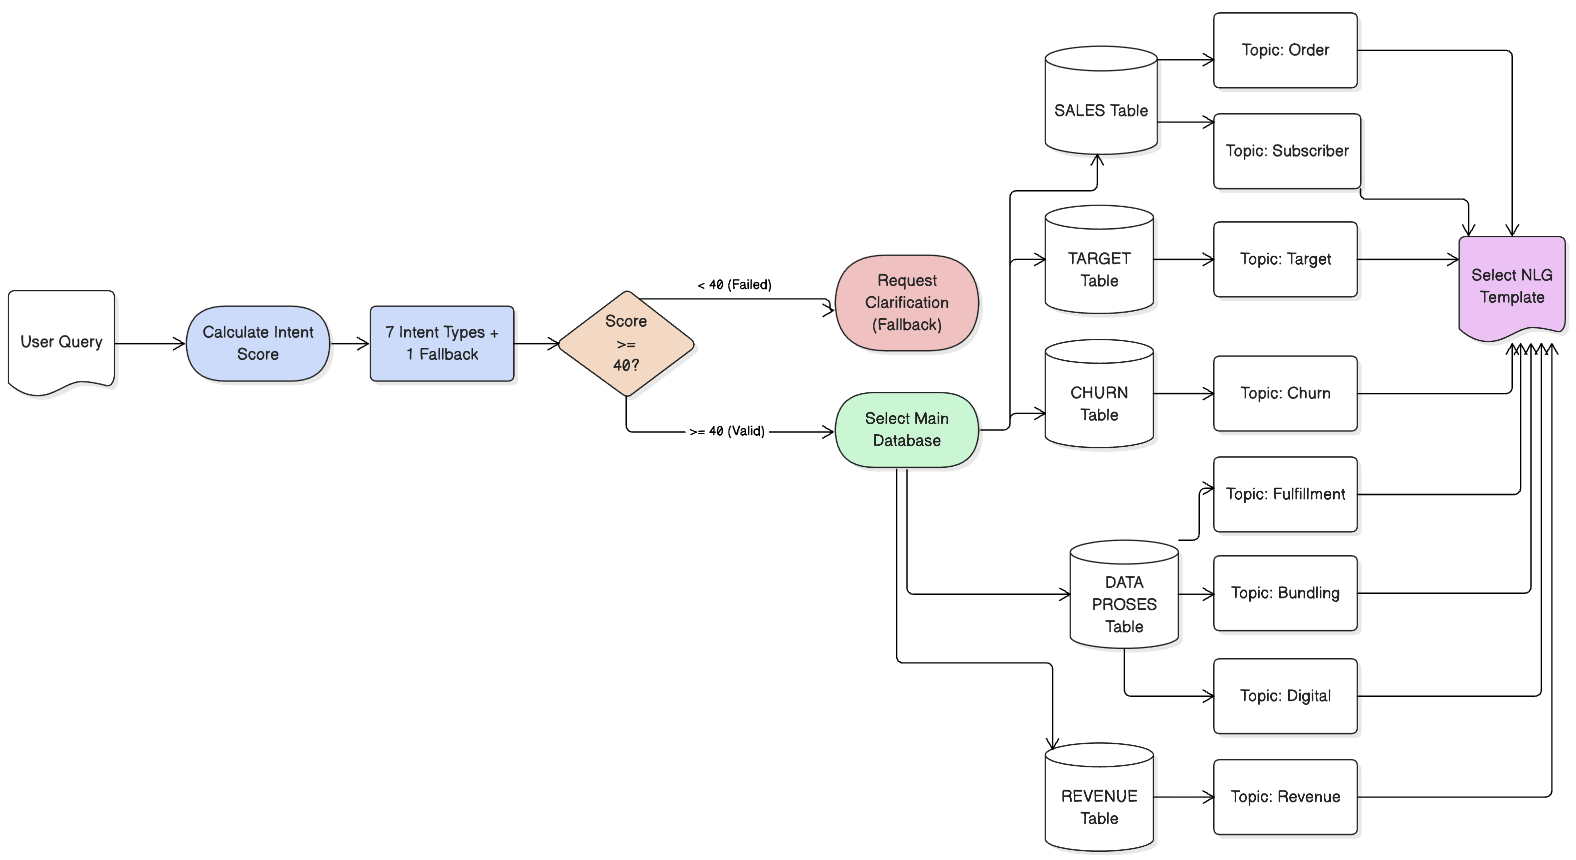
\includegraphics[width=\linewidth,height=4.8cm,keepaspectratio]{ars2.png}}
\caption{The internal architecture detailing the NLU mapping and core sublayers.}
\label{fig:ars2}
\vspace{-0.3cm}
\end{figure}

As illustrated in Fig.~\ref{fig:ars2}, the NLU Sublayer processes the user's raw input. To satisfy strict enterprise requirements for 100\% factual accuracy, the system avoids stochastic LLMs for data retrieval \cite{mulyatun2021chatbot}, employing a deterministic, confidence-weighted intent classifier instead. Upon classification, the query routes to the Core Sublayer. Here, the Analytics Engine executes the SQL query against the Oracle Database (Database Layer). For future projections, data is processed by the Forecasting Service (an independent Python/FastAPI microservice). Finally, the NLG Service synthesizes the outputs into natural language. Decoupling these machine learning operations ensures they do not block the application server.

\section{Methodology}
This research adopts the Cross-Industry Standard Process for Data Mining (CRISP-DM) framework. The methodology initiates with \textbf{Business and Data Understanding} to identify enterprise BI bottlenecks, followed by \textbf{Data Preparation} from Oracle schemas. The core technical development lies within the \textbf{Modeling and Evaluation} phases, encompassing the intent mapping and predictive forecasting components detailed below. Finally, the \textbf{Deployment} phase integrates these components into the BrightAI microservices.

\subsection{Intent Classification and Rule Mapping}
The NLU Sublayer encompasses 38 analytical rules mapped to five Oracle schemas. When a query is received, the algorithm evaluates the input against all rules, computing a Confidence Score ($C$) \cite{khosla2022evaluating}. Each rule defines a set of primary ($P$) and supporting ($S$) keywords. The Confidence Score is defined as a piecewise function where a primary keyword guarantees a base score of 80, further incremented by supporting keywords:

\begin{equation}
C = \begin{cases} 
\min(80 + P \cdot 10 + S \cdot 3, 100), & \text{if } P > 0 \\
65 + S \cdot 4, & \text{if } P = 0 \text{ and } S \ge 3 \\
0, & \text{otherwise}
\end{cases}
\end{equation}

To rigorously evaluate the classification efficiency of this NLU model, we utilize a confusion matrix. The matrix variables are defined for the chatbot as follows: True Positives ($TP$) represent correctly classified intents, True Negatives ($TN$) represent correctly rejected irrelevant intents, False Positives ($FP$) represent queries incorrectly assigned to a rule, and False Negatives ($FN$) represent valid queries the system failed to classify. The four fundamental evaluation metrics are explicitly formulated below:

\textbf{1. Accuracy:} Measures the overall correctness of the intent classification.
\begin{equation}
Accuracy = \frac{TP + TN}{TP + TN + FP + FN}
\end{equation}

\textbf{2. Precision:} Measures the exactness of the model; out of all queries assigned to a specific rule, how many actually belonged there.
\begin{equation}
Precision = \frac{TP}{TP + FP}
\end{equation}

\textbf{3. Recall:} Measures the completeness; out of all queries that should have triggered a rule, how many were successfully captured.
\begin{equation}
Recall = \frac{TP}{TP + FN}
\end{equation}

\textbf{4. F1-Score:} The harmonic mean of Precision and Recall, providing a balanced metric for uneven class distributions.
\begin{equation}
F1\ Score = 2 \times \frac{Precision \times Recall}{Precision + Recall}
\end{equation}

\subsection{Time Series Forecasting Models: Theoretical Basis}
The analytical layer evaluates four forecasting architectures \cite{sunendar2025comparison}. The selection of these four distinct methodologies serves specific empirical purposes:
1. \textbf{ARIMA} serves as a rigorous statistical baseline designed for linear, stationary data modeling.
2. \textbf{Facebook Prophet} is specifically designed to excel on datasets with powerful underlying business seasonality and holiday anomalies.
3. \textbf{LSTM} represents state-of-the-art deep learning, employed for its capability to decipher deeply embedded, complex non-linear relationships across long temporal sequences.
4. \textbf{GRU} provides a computationally streamlined alternative to LSTM, preventing overfitting on shorter, highly volatile enterprise datasets.

The mathematical formulations for these models are detailed below:

\textbf{1. AutoRegressive Integrated Moving Average (ARIMA):}
A classical statistical model relying on historical lags and forecast errors, formally denoted as $ARIMA(p, d, q)$, where $y'_t$ is the differenced series, $c$ is a constant, $\phi, \theta$ are AR/MA parameters, and $\epsilon_t$ is white noise:
\begin{equation}
y'_t = c + \phi_1 y'_{t-1} + \dots + \phi_p y'_{t-p} + \theta_1 \epsilon_{t-1} + \dots + \theta_q \epsilon_{t-q} + \epsilon_t
\end{equation}

\textbf{2. Facebook Prophet:}
An additive regression model optimized for business time series featuring strong seasonality, where $g(t)$ is the trend, $s(t)$ is periodic seasonality, $h(t)$ is holiday effects, and $\epsilon_t$ is the error term:
\begin{equation}
y(t) = g(t) + s(t) + h(t) + \epsilon_t
\end{equation}

\textbf{3. Long Short-Term Memory (LSTM):}
A sophisticated Recurrent Neural Network (RNN) designed to circumvent the vanishing gradient problem via cell states ($C_t$) and gates (forget $f_t$, input $i_t$, output $o_t$), where $W, b$ are weights/biases, $h_{t-1}$ is the previous state, $x_t$ is the input, and $\sigma$ is the sigmoid function:
\begin{equation}
\begin{aligned}
f_t &= \sigma(W_f \cdot [h_{t-1}, x_t] + b_f) \\
C_t &= f_t \ast C_{t-1} + i_t \ast \tanh(W_C \cdot [h_{t-1}, x_t] + b_C) \\
h_t &= o_t \ast \tanh(C_t)
\end{aligned}
\end{equation}

\textbf{4. Gated Recurrent Unit (GRU):}
A computationally streamlined variant of the LSTM, merging the forget and input gates into a single update gate ($z_t$) and employing a reset gate ($r_t$) with $\tilde{h}_t$ as the candidate hidden state:
\begin{equation}
\begin{aligned}
z_t &= \sigma(W_z \cdot [h_{t-1}, x_t]) \\
h_t &= (1 - z_t) \ast h_{t-1} + z_t \ast \tilde{h}_t
\end{aligned}
\end{equation}

\textbf{5. Baseline Model (Seasonal Naive):}
For rigorous relative evaluation, all models are benchmarked against a seasonal naive approach: $\hat{y}_{t+h} = y_{t+h-m(k+1)}$, where $m$ is the seasonal period and $k$ represents the completed seasonal cycles prior to the forecast horizon $h$.

\subsection{User Interface and Template-Based NLG}
To strictly mitigate hallucination risks, the system ensures all generated insights, including session contexts and metadata, are deterministically extracted from the Enterprise Data Warehouse (EDW). Furthermore, to validate operational efficacy, a subjective user evaluation was conducted using a 5-point Likert scale across four critical dimensions: 1) Factual Accuracy (alignment with EDW records), 2) Narrative Clarity (comprehensibility for corporate users), 3) Usability (interface intuitiveness), and 4) Analytical Relevance (contextual alignment with user queries).

\subsection{Evaluation Metrics and Mathematical Framework}
To ensure the empirical validity of the models, a rigorous dual-protocol methodology is applied: Chronological Holdout Validation (80/20) and Rolling-origin Cross-validation (walk-forward). The evaluation architecture comprehensively spans NLU matching precision, NLG narrative generation fidelity, and forecasting error minimization. Model efficacy is quantified using standard metrics such as Mean Absolute Error (MAE) and Root Mean Square Error (RMSE):

\textbf{1. Mean Absolute Error (MAE):} $MAE = \frac{1}{n}\sum_{t=1}^{n}|y_t - \hat{y}_t|$

\textbf{2. Root Mean Square Error (RMSE):} $RMSE = \sqrt{\frac{1}{n}\sum_{t=1}^{n}(y_t - \hat{y}_t)^2}$

where $y_t$ represents the actual observed value, $\hat{y}_t$ denotes the forecasted value, and $n$ is the total number of observations.

To evaluate scale-independent performance across different business domains, we utilize sMAPE and MASE:

\textbf{3. symmetric Mean Absolute Percentage Error (sMAPE):} $sMAPE = \frac{100\%}{n}\sum_{t=1}^{n}\frac{|y_t - \hat{y}_t|}{(|y_t| + |\hat{y}_t|)/2}$

\textbf{4. Mean Absolute Scaled Error (MASE):} $MASE = \frac{MAE_{Model}}{MAE_{Baseline}}$

Furthermore, the \textbf{Skill Score} quantifies the relative improvement over the seasonal baseline \cite{sirisha2022profit}:

\textbf{5. Skill Score:} $Skill\ Score = 1 - \frac{MAE_{Model}}{MAE_{Baseline}}$

\section{Implementation and Results}

\subsection{Frontend Layer: User Interface and Access}
The integrated frontend serves as the primary access point for stakeholders. As illustrated in Fig.~\ref{fig:hasil1}, the system employs a secure login page that authenticates corporate users prior to granting access to sensitive enterprise data. 

\begin{figure}[htbp]
\centerline{
\includegraphics[width=\linewidth,height=4.8cm,keepaspectratio]{hasil1.png}}
\caption{The secure BrightAI login page for enterprise user authentication.}
\label{fig:hasil1}
\vspace{-0.3cm}
\end{figure}

Upon successful authentication, the user accesses the primary conversational interface. As illustrated in Fig.~\ref{fig:hasil2}, the Chatbot Page provides an intuitive, messaging-style layout where executives submit natural language queries to immediately receive structured tabular data and factual narratives. Internal stakeholders gave the frontend a perfect score of \textbf{5.00} for Ease of Use, validating the intuitive flow.

It is important to acknowledge that the user interfaces depicted in both Fig.~\ref{fig:hasil1} and Fig.~\ref{fig:hasil2} are deliberately presented in the Indonesian language. This localized design directly reflects the operational constraints and the specific language requirements mandated by this thesis project, ensuring the system aligns with the enterprise's domestic stakeholder environment.

\begin{figure}[htbp]
\centerline{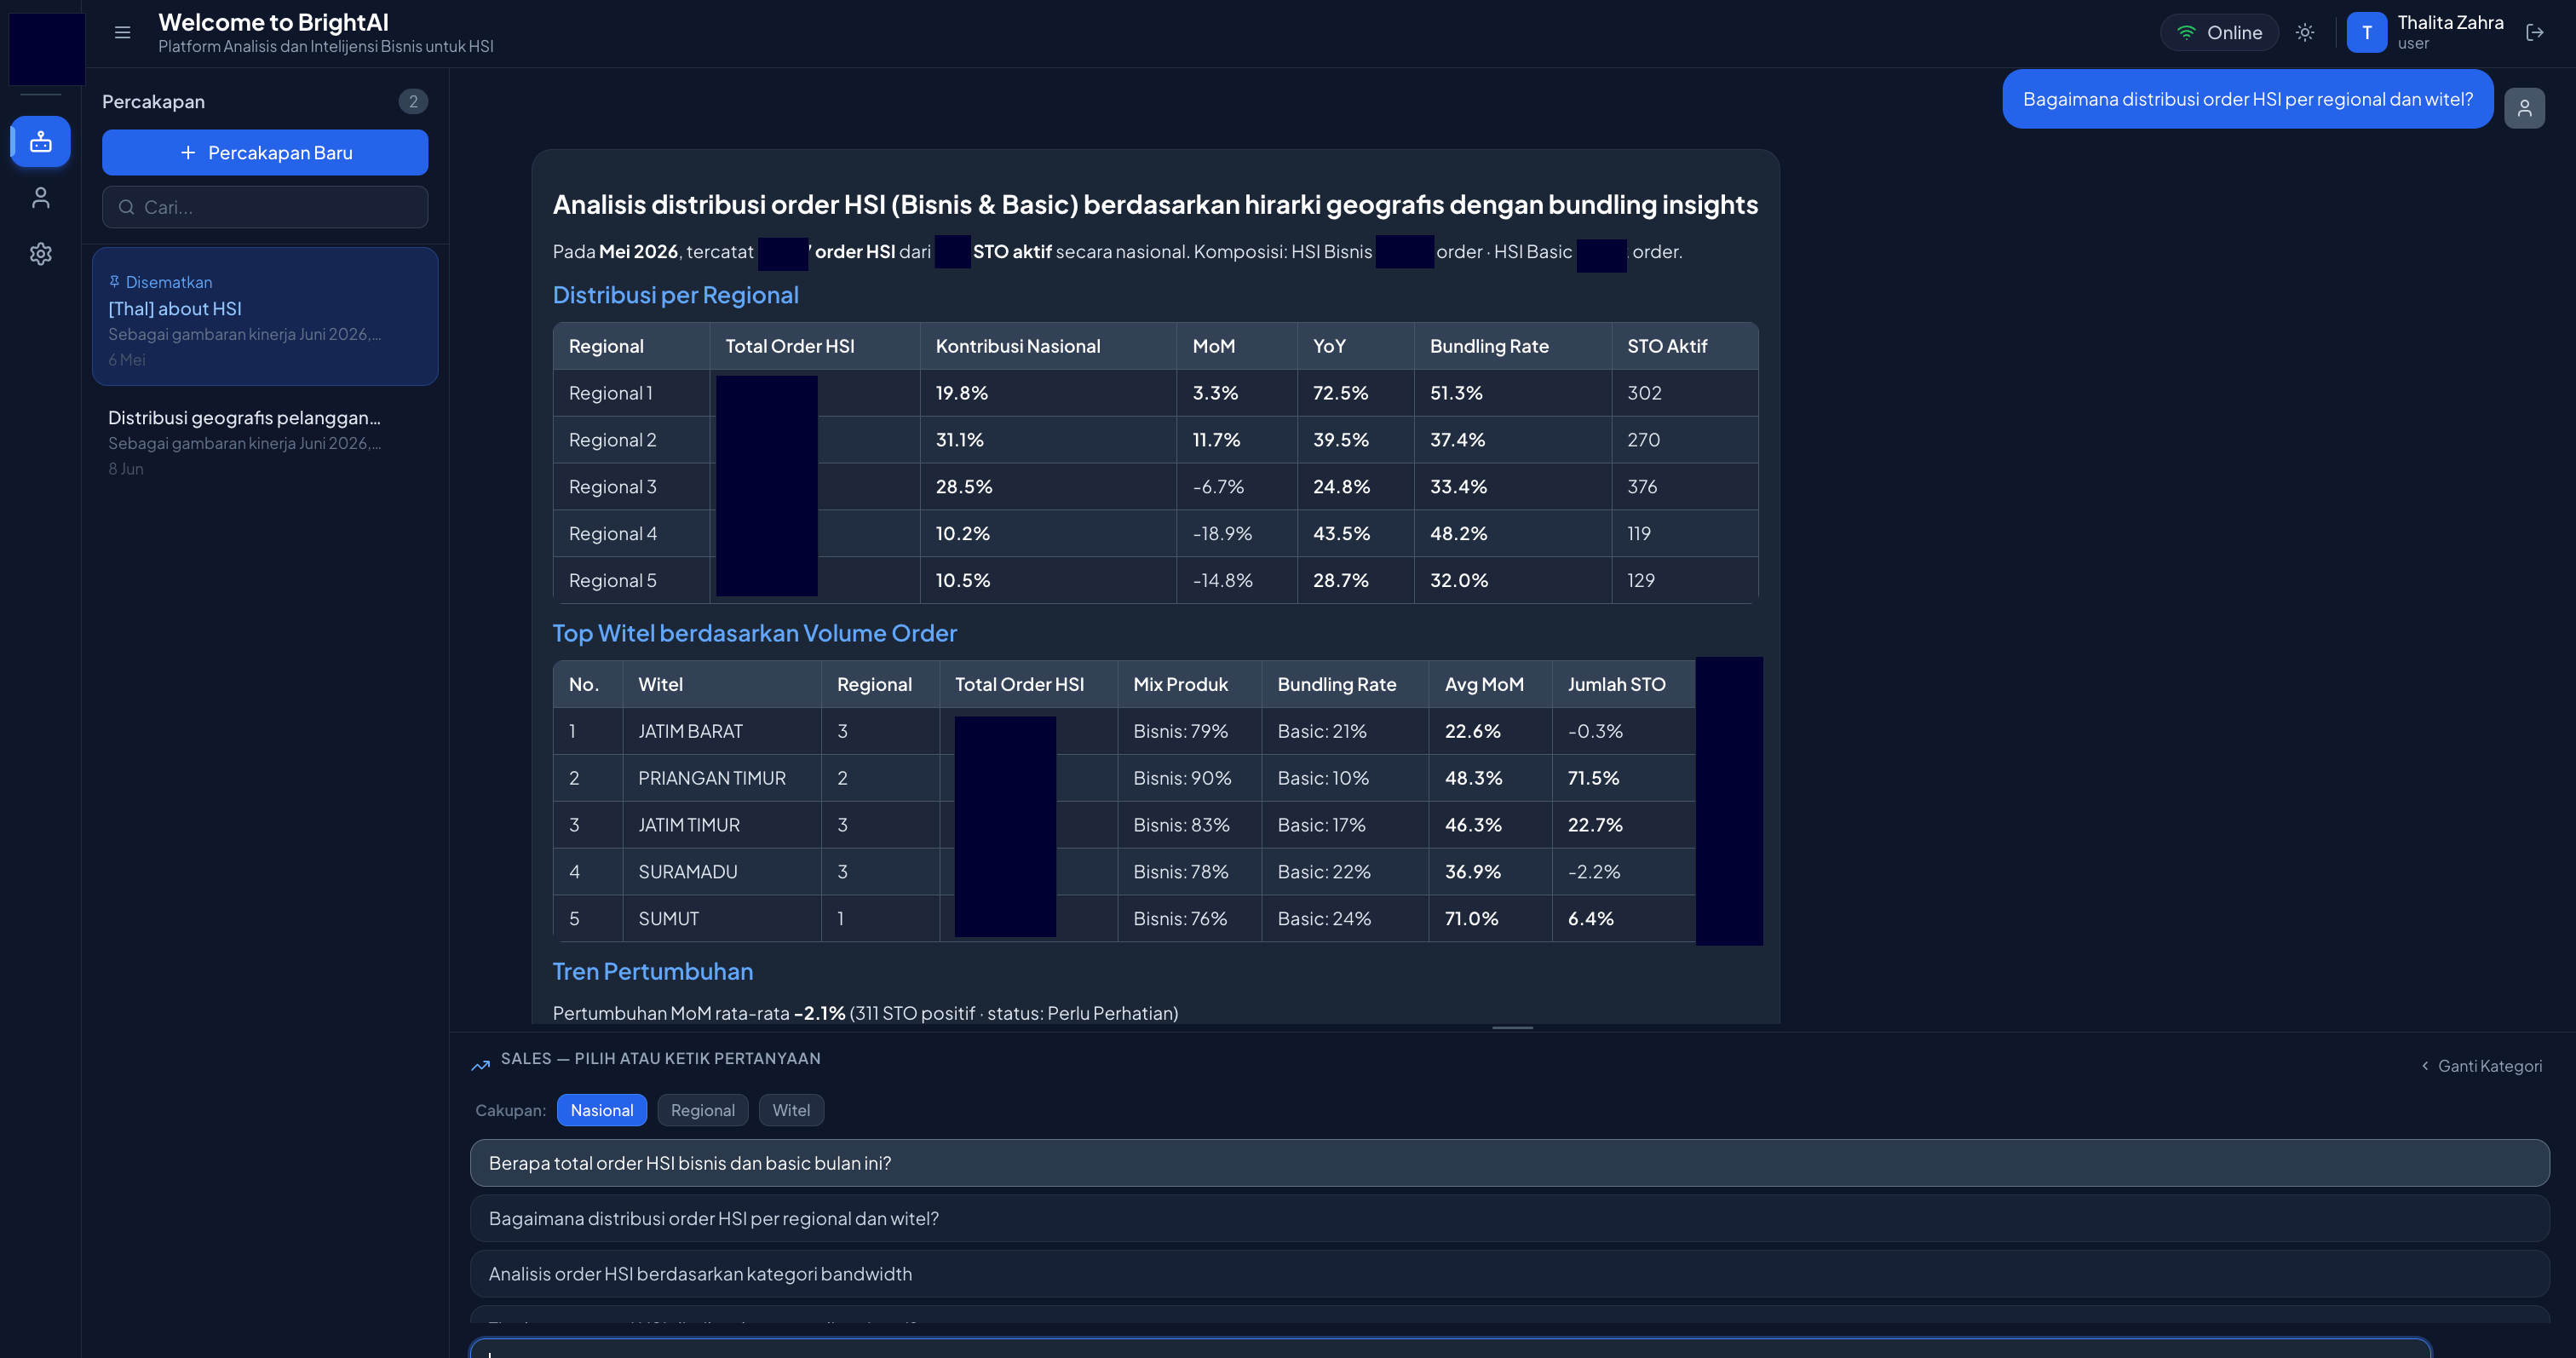
\includegraphics[width=\linewidth,height=4.8cm,keepaspectratio]{hasil2.png}}
\caption{The main BrightAI chatbot interface rendering structured tabular data.}
\label{fig:hasil2}
\vspace{-0.3cm}
\end{figure}

As visibly demonstrated in the chatbot interface above, the displayed textual narratives and structured tabular outputs are entirely generated by the BrightAI system. By seamlessly integrating the Natural Language Generation (NLG) engine with the EDW, the AI autonomously synthesizes raw database metrics into comprehensive, human-readable analytical insights in real-time.

\subsection{Backend Layer: NLU and Latency Performance}
During operational testing, 93\% of natural language queries successfully achieved a Confidence Score exceeding the baseline threshold of 40. This subset was subsequently evaluated to verify correct rule mapping. Initial NLU iterations exhibited a 90\% accuracy rate due to cross-domain keyword overlap. However, accuracy improved through rule-based heuristics. As detailed in Table~\ref{tab:nlu}, by implementing three disambiguation mechanisms---(1) \textit{Contextual Hard Gate}, (2) \textit{Cross-Domain Penalty}, and (3) \textit{Specific Phrase Bonus}---the NLU classification accuracy, precision, and recall reached \textbf{100\%} (1.000 F1-Score) across all 38 rules. Intents evaluated in $<1$ ms; rule matching executed in $<10$ ms.

\begin{table}[htbp] \footnotesize
\caption{Rule Matching Evaluation Metrics (NLU)}
\begin{center}
\begin{tabular}{lccc}
\toprule
\textbf{Aggregation Strategy} & \textbf{Precision} & \textbf{Recall} & \textbf{F1-Score} \\
\midrule
Macro & 1.000 & 1.000 & 1.000 \\
Weighted & 1.000 & 1.000 & 1.000 \\
Micro & 1.000 & 1.000 & 1.000 \\
\bottomrule
\end{tabular}
\label{tab:nlu}
\end{center}

\end{table}
\vspace{-0.3cm}

\subsection{Backend Layer: NLG Factual Accuracy}
The NLG module achieved 100\% factual accuracy. By piping quantitative data directly from the EDW into static templates, data hallucination risks are eliminated \cite{Celikyilmaz2020EvalTextGen}. 

As detailed in Table~\ref{tab:user_eval}, success was measured subjectively by the end-users across the four predefined dimensions, achieving an overall average score of \textbf{4.75 out of 5.00}. The system scored perfectly (5.00) in Response Accuracy, Narrative Clarity, and Ease of Use.

\begin{table}[htbp] \footnotesize
\caption{User Evaluation Scores per Quality Dimension}
\begin{center}
\begin{tabular}{lc}
\toprule
\textbf{Quality Dimension} & \textbf{Score (1-5)} \\
\midrule
Response Accuracy & 5 \\
Narrative Clarity & 5 \\
Ease of Use & 5 \\
Analysis Relevance & 4 \\
\midrule
\textbf{Average Score} & \textbf{4.75} \\
\bottomrule
\end{tabular}
\label{tab:user_eval}
\end{center}

\end{table}
\vspace{-0.3cm}

\subsection{Backend Layer: Forecasting Outcomes}
Walk-forward validation extracted precise scale-independent error metrics across four defining business domains.

\textbf{1. Order Metric Evaluation:} Table~\ref{tab:fc_order} details the performance of the models regarding internet service sales volume. The \textbf{GRU} architecture emerged as the most robust model for the Order Metric, achieving the lowest sMAPE (13.09\%) and the highest Skill Score (0.247). While all models technically satisfied the KPI thresholds (sMAPE $<30\%$), GRU's streamlined deep learning architecture proved effective in mitigating overfitting on relatively short, volatile enterprise data streams. Prophet also performed competitively, demonstrating that order data possesses strong underlying seasonal trends.

\begin{table}[htbp] \footnotesize
\caption{National Evaluation: Order Metric}
\begin{center}
\begin{tabular}{lcccc}
\toprule
\textbf{Model} & \textbf{sMAPE (\%)} & \textbf{MASE} & \textbf{Skill Score} & \textbf{KPI} \\
\midrule
\textbf{GRU} & \textbf{13.09} & \textbf{0.418} & \textbf{0.247} & \textbf{PASS} \\
LSTM & 16.50 & 0.521 & 0.063 & PASS \\
ARIMA & 16.74 & 0.538 & 0.032 & PASS \\
Prophet & 15.27 & 0.534 & 0.039 & PASS \\
\bottomrule
\end{tabular}
\label{tab:fc_order}
\end{center}

\end{table}
\vspace{-0.3cm}

\textbf{2. Churn Metric Evaluation:} Customer Churn (Table~\ref{tab:fc_churn}) demonstrated extreme data volatility driven by non-seasonal anomalies such as sudden promotional shifts \cite{Mena2023}. \textbf{GRU} retained its position as the premier model, securing an sMAPE of 22.29\%. Crucially, Prophet significantly underperformed in this evaluation (sMAPE 45.15\%, Skill Score -1.627). This outcome underscores that classical additive models fundamentally break down when forced to predict non-linear operational dynamics that lack a predictable seasonal calendar.

\begin{table}[htbp] \footnotesize
\caption{National Evaluation: Customer Churn Metric}
\begin{center}
\begin{tabular}{lcccc}
\toprule
\textbf{Model} & \textbf{sMAPE (\%)} & \textbf{MASE} & \textbf{Skill Score} & \textbf{KPI} \\
\midrule
\textbf{GRU} & \textbf{22.29} & \textbf{0.504} & \textbf{0.169} & \textbf{PASS} \\
LSTM & 22.97 & 0.516 & 0.149 & PASS \\
ARIMA & 26.53 & 0.596 & 0.017 & PASS \\
Prophet & 45.15 & 1.592 & -1.627 & FAIL \\
\bottomrule
\end{tabular}
\label{tab:fc_churn}
\end{center}

\end{table}
\vspace{-0.3cm}

\textbf{3. Target Realization Metric Evaluation:} Table~\ref{tab:fc_realisasi} outlines the forecasting accuracy regarding corporate sales target realizations. In forecasting medium-term target realization, deep learning models demonstrated superior performance. \textbf{LSTM} delivered high accuracy with an sMAPE of just 6.48\% and an outstanding Skill Score of 0.593. Because target realization data inherently contains clear medium-term structural trends, LSTM's sophisticated memory cell gates could successfully decipher those deep temporal dependencies without succumbing to statistical noise.

\begin{table}[htbp] \footnotesize
\caption{National Evaluation: Target Realization Metric}
\begin{center}
\begin{tabular}{lcccc}
\toprule
\textbf{Model} & \textbf{sMAPE (\%)} & \textbf{MASE} & \textbf{Skill Score} & \textbf{KPI} \\
\midrule
GRU & 8.27 & 0.101 & 0.481 & PASS \\
\textbf{LSTM} & \textbf{6.48} & \textbf{0.079} & \textbf{0.593} & \textbf{PASS} \\
ARIMA & 20.29 & 0.251 & -0.080 & PASS \\
Prophet & 12.36 & 0.157 & 0.193 & PASS \\
\bottomrule
\end{tabular}
\label{tab:fc_realisasi}
\end{center}

\end{table}
\vspace{-0.3cm}

\textbf{4. Average Install Days Evaluation:} For heavily stable, non-volatile operational logistics metrics such as average installation duration (Table~\ref{tab:fc_install}), classical statistical approaches proved remarkably resilient. \textbf{ARIMA} secured the highest overall ranking (sMAPE 10.75\%, Skill Score 0.480), outperforming the deep learning models. Prophet, inversely, showed significant performance degradation (sMAPE 176.92\%), reinforcing its inadequacy for steady-state data lacking strong, recurrent business holidays or weekly cycles. 

\begin{table}[htbp] \footnotesize
\caption{National Evaluation: Average Install Days}
\begin{center}
\begin{tabular}{lcccc}
\toprule
\textbf{Model} & \textbf{sMAPE (\%)} & \textbf{MASE} & \textbf{Skill Score} & \textbf{KPI} \\
\midrule
GRU & 10.86 & 0.020 & 0.400 & PASS \\
LSTM & 12.18 & 0.023 & 0.350 & PASS \\
\textbf{ARIMA} & \textbf{10.75} & \textbf{0.018} & \textbf{0.480} & \textbf{PASS} \\
Prophet & 176.92 & 1.124 & -10.00 & FAIL \\
\bottomrule
\end{tabular}
\label{tab:fc_install}
\end{center}

\end{table}
\section{Conclusion}
First, the decoupled three-tier architecture resolved manual business intelligence dependencies by providing a real-time conversational interface. This decoupling ensured predictive computations did not impede interface responsiveness.

Second, the NLU module achieved \textbf{100\% accuracy} across 38 analytical rules via contextual heuristics, successfully automating complex SQL query generation.

Third, the template-based NLG module guaranteed factual reliability. By mapping database returns into deterministic templates, the system eradicated hallucination risks inherent in generative LLMs.

Fourth, forecasting models were evaluated against KPIs: sMAPE $<30\%$, MASE $<1.0$, and Skill Score $>-0.1$. Absolute metrics (MAE, RMSE) were reported complementarily. Empirical results confirmed GRU, LSTM, and ARIMA met all operational thresholds (status: \textbf{PASS}). Conversely, Prophet failed (status: \textbf{FAIL}) due to algorithmic assumptions misaligned with data volatility. GRU delivered the optimal balance of predictive accuracy and computational stability. Finally, with a User Evaluation score of 4.75/5.00, BrightAI demonstrably democratizes data accessibility and accelerates strategic decision-making.

\begin{thebibliography}{00} \footnotesize
\bibitem{gul2023from} R. Gul and M. A. S. Al-Faryan, ``From insights to impact: leveraging data analytics for data-driven decision-making and productivity in banking sector,'' \textit{Humanities and Social Sciences Communications}, vol. 10, pp. 1--12, 2023.
\bibitem{shah2025hybrid} N. Shah, ``Hybrid Analytics Architecture: Integrating Traditional BI with AI-Powered Insights,'' \textit{World Journal of Advanced Engineering Technology and Sciences}, vol. 14, no. 2, pp. 256--271, 2025.
\bibitem{mulyatun2021chatbot} Mulyatun, D. Kurniawan, and A. Hudaya, ``Pendekatan Natural Language Processing pada Aplikasi Chatbot sebagai Alat Bantu Customer Service,'' \textit{Journal of Information System Management (JOISM)}, vol. 2, no. 2, pp. 12--17, 2021.
\bibitem{khosla2022evaluating} S. Khosla \textit{et al.}, ``Evaluating the Practical Utility of Confidence-score based Techniques for Unsupervised Open-World Classification,'' in \textit{Proc. of the Third Workshop on Insights from Negative Results in NLP}, 2022, pp. 20--28.
\bibitem{sunendar2025comparison} A. Sunendar, S. Wibirama, and N. A. Setiawan, ``Comparison of ARIMA, LSTM, and GRU Models for Sales Prediction in Indonesian Banking Stock Market,'' \textit{PILAR: Physics, Informatics, and Applied Research}, vol. 3, no. 1, pp. 67--78, 2025.
\bibitem{sirisha2022profit} U. M. Sirisha, M. C. Belavagi, and G. Attigeri, ``Profit Prediction Using ARIMA, SARIMA and LSTM Models in Time Series Forecasting: A Comparison,'' \textit{Int. Journal of Current Research and Review}, vol. 14, no. 24, pp. 32--42, 2022.
\bibitem{Mena2023} G. Mena \textit{et al.}, ``Exploiting Time-Varying RFM Measures for Customer Churn Prediction with Deep Neural Networks,'' \textit{Annals of Operations Research}, vol. 339, pp. 765--787, 2024.
\bibitem{Celikyilmaz2020EvalTextGen} A. Celikyilmaz, E. Clark, and J. Gao, ``Evaluation of Text Generation: A Survey,'' \textit{arXiv preprint arXiv:2006.14799}, 2020.
\end{thebibliography}

\end{document}
